%!TEX root = ../main.tex

\chapter{Presentation of the project}

Type providers have significant benefits that are worth exploring in other programming languages. I have created a project that aims to approximate the benefits of type providers in Rust.

The project is divided into five crates, as well as a crate demonstrating the use of the main crate. Most important of these are one library -- a procedural macro -- and two binaries -- a command line interface and a web interface. Figure~\ref{fig:crates} shows how the crates depend on each other.

\begin{figure}[ht!]
\vspace{2mm}
\centering
\begin{tikzpicture}[>=stealth, thick, shorten >=1pt]
\graph [layered layout, grow=up, level distance=1.3cm, nodes={draw, rectangle, rounded corners}] {
"json\_typegen\_demo" -> "json\_typegen";
"json\_typegen" -> "json\_typegen\_derive";
"json\_typegen\_derive" ->[shorten >=6pt] "json\_typegen\_shared";
"json\_typegen\_cli" -> "json\_typegen\_shared";
"json\_typegen\_web" ->[shorten >=6pt] "json\_typegen\_shared";
};
\end{tikzpicture}
\vspace{2mm}
\caption{Internal dependencies in the project}
\label{fig:crates}
\end{figure}

\section{The procedural macro}

The crate «json_typegen» provides a procedural macro of the same name, ‹json_typegen›. This macro provides an interface very similar to the type providers from \fsharpdata.

\begin{listing}[ht!]
\begin{minted}{rust}
#[macro_use]
extern crate json_typegen;
extern crate serde_json;

json_typegen!("Point", r#"{ "x": 1, "y": 2 }"#);

fn main() {
    let mut p: Point =
        serde_json::from_str(r#"{ "x": 3, "y": 5 }"#).unwrap();
    println!("deserialized = {:?}", p);
    p.x = 4;
    let serialized = serde_json::to_string(&p).unwrap();
    println!("serialized = {}", serialized);
}
\end{minted}
\caption{Usage of the procedural macro}
\label{lst:proc-macro-example}
\end{listing}

In listing~\ref{lst:proc-macro-example} a minimal example of usage of the procedural macro ‹json_typegen› is shown. This example is provided in the project source as a demo crate, «json_typegen_demo». It is worth noting that the calls to ‹unwrap› unwraps result values assuming success, and will crash the program in the event of a serialization or deserialization failure. In a real world use case we would replace these calls with error handling code.

As can be seen in the example, the procedural macro defines a type -- ‹Point› -- which is then available to be used by the programmer as any other type. The type gives type safe access to its fields, in the example ‹p.x›. Attempts to access an invalid field -- e.g. ‹p.z› -- would be a type error and thus be caught at compile time.

The procedural macro supports inline samples as shown, samples stored as local files and URLs that point to remote samples.

\begin{listing}[ht!]
\textbf{Invocation of procedural macro:}
\begin{minted}{rust}
json_typegen!("Point", r#"{ "x": 1, "y": 2 }"#);
\end{minted}
\vspace{5mm}

\textbf{Generated code:}
\begin{minted}{rust}
#[derive(Default, Debug, Clone, PartialEq,
         Serialize, Deserialize)]
struct Point {
    x: i64,
    y: i64,
}
\end{minted}
\caption{The code generated by a macro invocation}
\label{lst:basic-macro-output}
\end{listing}

Based on the JSON samples, types are inferred and Rust code with type declarations is generated. Listing~\ref{lst:basic-macro-output} shows the code generated by the macro shown in the example in listing~\ref{lst:proc-macro-example}. The types generated by «json_typegen» are all built up from the same base Rust types:

\begin{itemize}
  \item ‹Vec<T>›, growable arrays, and ‹Option<T>›, optional values, with the type parameter ‹T› always being either another of our base types or an earlier generated type.
  \item ‹i64›, 64-bit integers, and ‹f64›, 64-bit floating point numbers
  \item ‹String›, heap-allocated strings
  \item ‹bool›, boolean values
  \item ‹serde_json::Value›, «serde_json»s catchall type, as a fallback when the inference gets either not enough or conflicting information
\end{itemize}

In chapter~\ref{sec:code-generation} we will look in more detail at how these types are inferred and how the types are generated.

\subsection{Limitations compared to an actual type provider}
\label{sec:macro-limitations}

While the procedural macro looks like and in many ways works like a type provider, it is not a real type provider. For some features actual support for type providers in the compiler and the tooling would be necessary.

At the moment there is no tooling solution for Rust that provides autocomplete for types generated by procedural macros. There is reason to believe that this may change in the future. However, if this will happen at all, if it would work for the ‹json_typegen› macro specifically and when it would hypothetically be done is all mostly guesswork at this point.

Since this solution is only a procedural macro that is run at compile time and does not have knowledge of the rest of the program there is no way to implement code generation on demand that depends on how the type is used. A version of this feature would be possible to do with a procedural macro system, but would require making significant changes to the Rust compiler. It is also very possible that it is not desirable to change the macro system in this manner.

\subsubsection{Procedural macro hack}

Another limitation of the current implementation is that the macro can only be used once per scope. This is a consequence of the fact that, at the time of writing, function-like procedural macros are currently not enabled on the stable version of the Rust compiler.

To work around this limitation ‹json_typegen› is actually a normal pattern based macro. The invocation of this macro expands to the declaration of a dummy type that uses a custom derive that is implemented in «json_typegen_derive»\footnote{This hack is demonstrated in isolation, and described in more detail at \url{https://github.com/dtolnay/proc-macro-hack}}. Due to a limitation in current pattern based macros the macro is unable to create new names for each dummy type. Because of this two invocations of the macro would create two (unused) types with the same name.

\begin{listing}[ht!]
\begin{minted}{rust}
mod point {
    json_typegen!("pub Point", "point_sample.json");
}

mod vector {
    json_typegen!("pub Vector", "vector_sample.json");
}

use point::*;
use vector::*;
\end{minted}
\caption{Workaround for the single use limitation imposed by the procedural macro hack}
\label{lst:hack-workaround}
\end{listing}

In my testing thus far I have not had a use case where I needed to work around this limitation. But if necessary the easiest way is to wrap the macro invocation in module scopes, and if desired import the created types. Another workaround is to use «json_typegen_derive» directly. However in the near future\footnote{Tracking issue for procedural macros: \url{https://github.com/rust-lang/rust/issues/38356}} no hack should be needed at all as function-like procedural macros become available on the stable compiler.

\section{The command line interface}

\begin{listing}[ht!]
\textbf{Invocation of procedural macro:}
\begin{minted}{rust}
json_typegen!("Point", r#"{ "x": 1, "y": 2 }"#);
\end{minted}
\vspace{5mm}

\textbf{Equivalent run of the CLI:}
\begin{minted}{shell}
json_typegen -n Point '{ "x": 1, "y": 2 }'
\end{minted}
\caption{Equivalent uses of CLI and macro}
\label{lst:cli-and-macro}
\end{listing}

The crate «json_typegen_cli» provides a binary, ‹json_typegen›, which is a command line interface (CLI) to the same code generation as is used in the procedural macro. In other words would running the binary ‹json_typegen› and invoking the macro ‹json_typegen› output the same code if given the same input sample and options.

% Diffing of earlier code with new

\section{The web interface}

\begin{figure}[ht!]
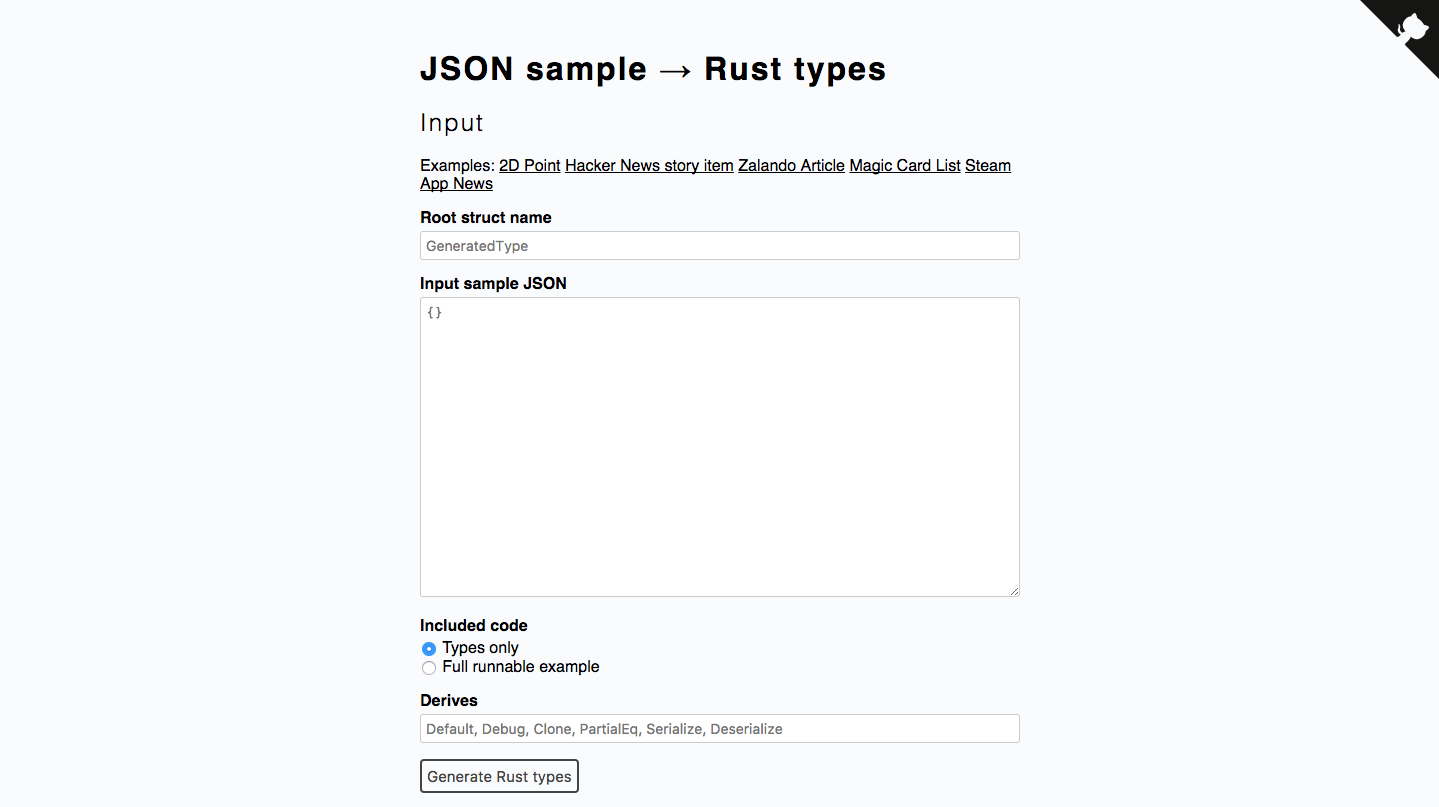
\includegraphics[width=\textwidth]{json_typegen_web}
\hspace*{-1.5in} % To get rid of some weird bottom margin
\caption{Screenshot of the web interface}
\label{fig:web-screenshot}
\end{figure}

The procedural macro and the command line interface both require the user to download and compile a somewhat significant amount of code. In small projects where the sample can be assumed not to change, this initial cost may for a lot of users seem to outweigh the benefits of the code generation.

Both of these kinds of interfaces also have a somewhat suboptimal user experience if the user wants to use a large number of configuration options. To counteract both of these problems I have made a web interface as a third way to use access the code generation logic.

The crate «json_typegen_web» provides a binary that both provides a web API for the code generation, as well as hosting the static HTML/JavaScript files providing a frontend to this API.

\section{Shared code}
\label{sec:shared-code}

As seen in figure~\ref{fig:crates} the macro, web interface and CLI all depend on a common crate, «json_typegen_shared». This crate contains the actual inference and code generation logic. The following general data flow is common to all three interfaces:

\begin{enumerate}
  \item Get the actual JSON text for the sample.
  \item Parse the JSON text into JSON values
  \item Infer type shapes from the JSON values
  \item Generate Rust code from the type shapes
\end{enumerate}

In the CLI and the web interface there is additionally a phase of formatting the generated code before the code is output to the user.

% FIXME: The rest of this section is basically just all wrong.
As mentioned in section~\ref{sec:macros} procedural macros are $ ‹TokenStream› \rightarrow ‹TokenStream› $ functions. However a ‹TokenStream› can both be parsed from a string, and written into a string. In other words we have access to both a $ ‹String› \rightarrow ‹TokenStream› $ and a $ ‹TokenStream› \rightarrow ‹String› $ function.

The different interfaces we want to provide place some requirements on what signatures we need to be able to use our code with. As mentioned, procedural macros need to have the signature $ ‹TokenStream› \rightarrow ‹TokenStream› $. A web API on the other hand must at least externally have an interface that boils down to $ ‹String› \rightarrow ‹String› $. That leaves us with two alternatives, (using $\rightarrow$ for a conversion and $\Rightarrow$ for the transformation):

\begin{align*}
‹String› \rightarrow ‹TokenStream› &\Rightarrow ‹TokenStream› \rightarrow ‹String› & \text{web} \\
                   ‹TokenStream› &\Rightarrow ‹TokenStream›                    & \text{macro} \\
\\
                        ‹String› &\Rightarrow ‹String›                         & \text{web} \\
‹TokenStream› \rightarrow ‹String› &\Rightarrow ‹String› \rightarrow ‹TokenStream› & \text{macro}
\end{align*}

In the real project things are a bit more complicated, as more types are involved, but the central point that we can consolidate different interfaces to a shared core that does the actual transformation thanks to conversion methods still stands.

\section{Synergy}
% Demonstrate how CLI or web interface can be used together with proc-macro. Explain how this then gives autocomplete etc.

Having these different interfaces provides us with some benefits that would be very difficult or impossible to achieve with only a single one.

With the three interfaces, there is a clear migration path for most use cases. A user can start with the web interface to test the code generation and see if the results fit their use case. Since it is just a normal website they can do this without having to install anything or add any dependencies.

If the code generation is suitable to their use case, copying and pasting from a website can get tedious. That combined with the additional benefits of the procedural macro will likely lead people to try the procedural macro.

As mentioned in section~\ref{sec:macro-limitations}, the procedural macro has some limitations, and as mentioned in section~\ref{sec:disadvantages-of-type-providers} even real type providers have their disadvantages. With a combination of the interfaces in this project, interesting solutions or workarounds for several of these issues are possible.

% FIXME: Unreadable sentence
Perhaps the most obvious concern that is no longer an issue is the fact that it is not possible to see expanded code with the type providers from \fsharpdata\ and the procedural macro in «json_typegen».
The two additional interfaces in this project both make it easy to see the generated code.\footnote{On nightly versions of Rust it is in fact also possible to see the resulting code after macro expansion. However, since it is fully expanded it is primarily useful for debugging purposes.}
% (also mention cargo-expand here)

The two additional interfaces also makes lock-in almost a non-issue. If a user wants to stop using «json_typegen» entirely, they can just do a final one time generation of the code. They can do this using either the web or command line interface, and replace the macro invocation with the generated code.

% autocomplete by generated code
One reason why someone might not want to use the procedural macro at the moment is the current lack of autocomplete. However, switching from the procedural macro to manually generated code means abandoning the verification against the external resource that the procedural macro gives.

\subsection{Conditional compilation}

% In Rust you can do conditional compilation by...
% #[cfg(feature = "online-samples")]
% Conditional compilation means that...

% autocomplete by generated code, but keeping benefits
To make the generated source available to editors while still keeping the benefits of the procedural macro it is possible to use conditional compilation. Listing~\ref{lst:conditional-compilation} shows an example setup where pre-generated code is used in the default build, but the pre-generated code is ignored and the procedural macro used instead when a compilation flag is enabled.

\begin{listing}[ht!]
\textbf{In the source code:}
\begin{minted}{rust}
#[cfg(not(feature = "online-samples"))]
#[derive(Default, Debug, Clone, Serialize, Deserialize)]
struct Point {
    x: i64,
    y: i64,
}

#[cfg(feature = "online-samples")]
json_typegen!("Point", "http://example.com/point.json");
\end{minted}
\vspace{5mm}

\textbf{Normal build:}
\begin{minted}{bash}
$ cargo build
\end{minted}
\vspace{5mm}

\textbf{Type checking against online samples:}
\begin{minted}{bash}
$ cargo check --features "online-samples"
\end{minted}
\caption{Conditional compilation}
\label{lst:conditional-compilation}
\end{listing}

% require network access only for verification
Using conditional compilation in this way also lets us get around the issue of requiring network access to build. If network access is the only issue we care about we don't even need to pre-generate the code, and can instead use two macro invocations -- one with a local or inline sample and one with the remote one -- as our two options.

% separate build for verification, so "normal" build still reproducible
Since the normal build in such a setup does not rely on an external resource we also get reproducible builds this way. Even if the external resource changes, it will still be possible to check out an old version of our source code and compile it. This can actually be very useful e.g. for tracking down bugs with tools like ‹git bisect›.

\section{Configurability}

There is one final problem that does not just apply to type provider like tools, but to code generation in general: Code generation always has to make some assumptions, and thus do not cover every use case and every requirement a programmer might have.

\begin{listing}[ht!]
\textbf{Sample:}
\begin{minted}{json}
{
  "registered": "2016-08-19",
  "..."
}
\end{minted}
\vspace{5mm}

\textbf{Inferred type:}
\begin{minted}{rust}
#[derive(...)]
struct Order {
    registered: String,
    ...
}
\end{minted}
\vspace{5mm}

\textbf{Desired type:}
\begin{minted}{rust}
#[derive(...)]
struct Order {
    registered: Date,
    ...
}
\end{minted}
\caption{A simple example of how generated code can fall short}
\label{lst:string-date}
\end{listing}

Listing~\ref{lst:string-date} shows a simple example of a case where the inferred type falls short of what the programmer would write by hand. There is no ‹Date› type in the Rust standard library, and as such, even with inspection of the ‹String› it would not be natural for the code generation to infer a ‹Date› type by default. While the ‹Date› type specifically may conceivably be added to the standard library in the future, the same example could apply to all manner of domain specific types.

In such cases where the generated code falls short the programmer has a few alternatives:

\begin{itemize}
  \item They can simply use the generated code as is, and convert from ‹String› to ‹Date› as necessary. If the suboptimal type is used frequently in the code though, littering the code with snippets like ‹Date::from(order.registered)› becomes frustrating pretty fast.
  \item They can customize the generated code by hand, and reapply the customizations whenever the code has to be generated again. Since this requires access to the generated code this alternative means abandoning any procedural macro or type provider. As it also makes the customized code incompatible with the generated code conditional compilation will not help here either.
  \item Finally, they can customize the generated code by hand, and completely abandon the code generation tool.
\end{itemize}

All of these alternatives have significant downsides, so if configuration of the code generation is possible, and does not come with significant downsides of its own it would in most cases be clearly preferable.

While it is clear that «json_typegen» should have at least \emph{some} configuration options, it is not obvious to what extent. It is probably not a good idea to try to cover every edge case, as such a goal could quickly lead the code to become too complex to maintain and expand. We can however make an effort to cover the most common cases, and thus increase the usefulness of the project for most people.

In the next sections I will discuss the configuration options currently available in «json_typegen» and some proposals for future expansions of these options.

\subsection{Visibility}

Perhaps the simplest configuration option in «json_typegen» is type visibility. By default the generated types have no visibility specification. In Rust this means that the types are private, i.e. only accessible from the module\footnote{A file in Rust is itself a module} they are defined in, and any modules it may contain.

Private visibility for types from «json_typegen» was chosen as the default because of the inherent volatility of generating types from external resources and the fact that any change to a public type is considered a breaking API change. Thus, if the types were public by default, any change in an external sample would cause a breaking API change in users crates. If this is what the users desires, they should be free to choose so, but it is not something that should happen by accident.

To set a more public visibility for the generated types, a visibility specifier may be given along with the name for the root type. E.g. ‹json_typegen!("pub Point", ...)› would create the type ‹Point› as a public type, and if the type name ‹"pub(crate) Point"› was given, it would be created as a type visible within the current crate.

By default in «json_typegen» struct fields \say{inherit} the visibility specifier (if any) of the containing struct. This should usually be the desired behavior, but if not it can be overridden with a visibility specifier set using the option ‹field-visibility›.

\subsection{Derive list}
\label{sec:derive-list}

As explained in section~\ref{sec:traits} common behavior is specified in traits, and many of these traits can be derived -- automatically implemented -- by annotating the type with a list of traits to derive.

By default «json_typegen» annotates each generated type with the following derive list:

\begin{minted}{rust}
#[derive(Default, Debug, Clone, PartialEq, Serialize, Deserialize)]
\end{minted}

In other words will every type generated by «json_typegen» implement every trait in this list. The derive list can be overridden with the ‹derives› option. None of the traits are mandatory, but a generated type with an empty derive list would be close to useless. Since each trait has a significant effect we will look at each of the default derived traits separately. Additionally we will look at some additional traits that can be derived that a user might want to add for different use cases.

% FIXME: Show testing (appendix?)
Any unused traits and the accompanying code is eliminated by compiler optimizations when doing release builds, and so do not contribute anything to binary size. The added code generation of unused traits added very slightly to compile time in my testing, but not enough so as to be noticeable.

Since the cost for additional derived traits is so small, all the traits that are implemented for our base types\footnote{As a reminder, our base types are ‹Vec<T>›, ‹Option<T>› ‹i64›, ‹f64›, ‹String›, ‹bool› and ‹serde_json::Value›, hereafter referred to as ‹JsonVal›.} are in our default list.

\subsubsection{Serialize, Deserialize}

‹Serialize› and ‹Deserialize› are as explained in section~\ref{sec:serde} the traits that lets «serde»-compatible libraries convert to and from their various formats. It may seem like you would always want these traits, as creating types that can be serialized and deserialized is kind of \say{the point} of «json_typegen». Indeed, one would almost always want to have at least one of these traits, and sometimes both, depending on the use case. As such, in the default list both are included, but when customizing, often one can eliminate one of them. % Why?

% Converting to other formats

\subsubsection{Default, Debug, Clone}

The «Default» trait provides a no-argument constructor, creating the default value for the type. Deriving this trait creates the no-argument constructor filling in the field values with their respective default values.

This trait is in the default list mostly because it is useful for quick testing and for examples, and as such is a good aid in explorative programming. For handwritten types it usually makes more sense to manually set the default values.

Implementing the ‹Debug› trait makes the type printable via the ‹?› and \icode{\#?} debug format specifiers. E.g. an instance ‹v› of a type that implements the ‹Debug› trait is a valid argument in a statement like ‹println!("{:?}", v);›. Without implementing this trait, instances of a type can not be directly printed.

The ‹Clone› trait makes it possible to make a copy of an instance of the type by calling the ‹clone› method. For the generated types the derived implementation will result in a deep copy, which relatively speaking will be expensive. This should usually be avoided in high performance code, but is sometimes unavoidable. In quick testing and explorative programming however, it can often be quicker and easier to clone rather than try to satisfy Rusts borrow checker.

\subsubsection{Eq, PartialEq}

‹Eq› and ‹PartialEq› implements methods for comparisons that are, respectively, full and partial equivalence relations. Implementing ‹PartialEq› makes it possible to use the ‹==› and ‹!=› operators. ‹Eq› provides no additional functionality, and is just a marker trait declaring the relation to be a full equivalence relation.

‹PartialEq› is implemented for all of our base types, and is as such included in the default derive list. ‹Eq› on the other hand is not implemented for ‹f64›, floating point numbers, and ‹JsonVal›, as they themselves can contain floating point numbers.

‹f64› does not implement ‹Eq› because one of the requirements of a full equivalence relation is that it is reflexive, i.e. that every value is equal to itself. The possibility of ‹NaN› values makes ‹f64› not satisfy this property, as ‹NaN != NaN›.

While ‹f64› should not be ‹Eq›, JSON numbers are actually not allowed to be NaN or Infinity according to RFC 7159\cite[7]{RFC7159}. This means that if we could guarantee that only values from JSON data is stored in any fields that are inferred as ‹f64› we could safely make them ‹Eq›. Unfortunately, this is not something we can guarantee in Rust as immutability is a property of variable bindings, and not on fields.

‹JsonVal› actually enforces that its numbers don't contain ‹Infinite› or ‹NaN› and thus \emph{could} be ‹Eq›.

Users that know they won't have any floats or inference issues that leads to ‹JsonVal› values can add ‹Eq› to the derive list. If they have floats or ‹JsonVal› values, but are sure that any floats will come from JSON, an ‹Eq› implementation can be manually added with a ‹impl Eq for TheType {}› for each generated type. If this is something many people would do, generating these lines is something that could somewhat easily be added to «json_typegen».

\subsubsection{Hash}

Like with ‹Eq›, ‹Hash› is implemented for all of our base types except ‹f64› and ‹JsonVal›. The problem here again is ‹NaN›, but it is not as clear cut as with ‹Eq›. There are several reasonable, but no perfect solution to how floats should be hashable, so the Rust standard library provides no ‹Hash› implementation for ‹f64›. Unfortunately this leaves us with users only being able to add ‹Hash› to the derive list when they have no floats or ‹JsonVal› values (or implementing ‹Hash› manually).

This lack of ‹Hash› and ‹Eq› means that types generated with the default configuration can not be entered into any ‹HashSet› and can not be used in keys in a ‹HashMap›.

\subsubsection{Ord, PartialOrd}

% PartialOrd missing for ‹serde_json::Value›

\subsubsection{New}

In addition to the derives provided the standard library and «serde»  (which we already assume as a peer dependency) there are other custom derive libraries that can be used to add functionality to the generated types from «json_typegen». One simple such example is the «derive-new» crate, which derives a ‹new› constructor for the type with all fields as arguments. To add this functionality to all the generated types, all a user of «json_typegen» has to do is to add «derive-new» as a dependency, and add ‹New› to the derive list.

\subsubsection{Frunk: Generic, LabelledGeneric}

I won't go into detail on all the different functionality that can be added by custom derives, but one library that is of particular interest to us is «frunk». «frunk» is a library for doing functional generic programming in Rust. Among the things that it provides are two traits and accompanying derives: ‹Generic› and ‹LabelledGeneric›.

% FIXME: Add nominal/structural typing to the introduction

As explained in section~\ref{sec:rust-intro} Rust is nominally typed. This means that if we create types that have the same shape, but different names, they can not be used in place of each other, and converting between them is not all that easy. While we will look at other ways around this issue as well, ‹Generic› and ‹LabelledGeneric› provide a way to get a semblance of structural typing in Rust.

Types that implement ‹Generic› can be converted between each other if they are structurally the same, i.e. if the types have the same number of fields, with the same types, in the same order. ‹LabelledGeneric› will additionally require the fields to have the same names to allow the conversion.

\subsection{JSON pointers}
\label{sec:json-pointers}

While some configuration options like type visibility and the derive list make sense to specify globally, for the whole JSON document at once, a lot of what would be beneficial to configure has to be done on a much more granular level.

The initial case in listing~\ref{lst:string-date}, where we would want the type of a specific field to be ‹Date› rather than the inferred ‹String› is an example of where we would need such granularity.

In the example we would want to target \say{the field ‹registered› of the root object}. In our original JSON example of section~\ref{sec:json} we extracted \say{the field ‹areaCode› of the first element of the ‹phoneNumbers› field of the root object}. One of the ways we did this was with the ‹pointer› method from «serde_json» which takes as an argument something called a JSON pointer.

The JSON Pointer specification\cite{RFC6901} was originally developed along with the specification for JSON Patch\cite{RFC6902} for the HTTP PATCH method, which needed a way to specify specific elements of a JSON document. A JSON pointer is simply a string consisting of \say{reference tokens} each prefixed with a forward slash (to separate the tokens). A reference token is interpreted as either a field name or an array index, depending on whether an object or an array is encountered. So to specify \say{the field ‹registered› of the root object} we would write the JSON pointer ‹"/registered"›. And the JSON pointer we used in section~\ref{sec:json} to extract \say{the field ‹areaCode› of the first element of the ‹phoneNumbers› field of the root object} was ‹"/phoneNumbers/0/areaCode"›.

Since JSON pointers are representable as simple strings they are easy to use as arguments to both macros or in command line invocations. Since they are already used by «serde_json» it also makes sense to use JSON pointers rather than introduce yet another way to reference data originating from JSON.

Since JSON pointers are a \say{stringly typed} way to talk about data, it may seem strange to use them in a project that is so focused on type safety. There is however a significant distinction in using such code at compile time and at runtime. The criticism of \say{stringly typed} code in a strongly typed language is that it ends up reverting to a state where errors are discovered at runtime. If configuration for «json_typegen» specified through a JSON pointer does not apply to any of the sample, this can be known well before runtime, when generating the code (i.e. at compile time for the macro), and a warning or an error can be shown to the user at that point in time.

% Actually show some examples of using JSON pointers for configuration

Due to the use case the JSON pointer specification was developed for, there is however a rather glaring omission when it comes to adapting it to our use case. The complete lack of any wildcard.

% Existing solutions to lack of wildcard

\placeholder{Configuration/inference hints through JSON pointers}

\subsection{Cost of configurability}

While extensive configurability has significant benefits, there are also significant costs. Every configuration option a project adds increases its exposed API surface. The more exposed API surface we have, the more difficult maintenance and continued development becomes with making breaking changes.

With multiple interfaces each added configuration option in the shared code also needs to be exposed and handled multiple times. E.g. for just the web interface, each option needs to be added to the HTML form, added to the communication with the backend and be handled by the backend. Then similar work has to be done for the command line interface and the procedural macro.

% Problems with adding a lot of configuration in a project with multiple interfaces

% Approaches to working around this by generating parts of the interfaces based on the Config data type.

\section{Improving the synergy}

While the synergy between the different interfaces is already quite good there are ways in which it could be improved.

Since many of the use cases involve moving between the interfaces, making the transition between them as smooth as possible is an important part of the total user experience of the project.

While the "native" user experiences of the interfaces are quite different, with different strengths and weaknesses, the central functionality they provide, including configurability, should be the same. However if a user have taken extensive advantage of this configurability, having to replicate the same configuration settings from one interface in another can erase the convenience the other interface would provide.

For example is one of the use cases for the web interface to easily be able to see the generated code when using the procedural macro. However, a option in the macro is expressed as code, while the natural interface for the website is a form. For this specific use case it would be much nicer to just be able to copy the macro invocation as text, and get the output without having to use the form. In other words would it be convenient if the web interface would be able to read the macro syntax as an additional input format. Use cases for the CLI would benefit much the same way if a macro invocation could be used directly to generate code. What I propose is essentially to use the macro syntax as an ad hoc configuration interchange format.

If the web interface additionally can output in the macro syntax we get easy transitions that cover what I think are the most likely user stories:

\begin{itemize}
  \item Just discovered the project, and having tested in web interface, want to start using the macro: web $\rightarrow$ macro.
  \item Using the macro, but want to see the generated code for quick debugging: macro $\rightarrow$ web.
  \item Using the macro, but want to use CLI for autocomplete or other reasons for conditional compilation: macro $\rightarrow$ CLI.
\end{itemize}

\begin{figure}[ht!]
\vspace{2mm}
\centering
\begin{tikzpicture}[>=stealth, thick, shorten >=1pt, node distance=3.5cm, auto, scale=3]
  \tikzstyle{every state}=[draw, minimum size=1.5cm]

  \node[state] (cli)   at (0,0)       {CLI};
  \node[state] (macro) at (1,0)       {macro};
  \node[state] (web)   at (0.5,0.866) {web};

  \path[->] (web) edge [bend right=20] (cli);
  \path[->] (web) edge [bend right=20] (macro);
  \path[->] (macro) edge [bend right=20] (cli);
  \path[->] (macro) edge [bend right=20] (web);
  \path[->, dashed] (cli) edge [bend right=20] (web);
  \path[->, dashed] (cli) edge [bend right=20] (macro);
\end{tikzpicture}
\vspace{2mm}
\caption{Transitions enabled by CLI and web interface being able to read, and web interface being able to write, macro syntax. The dashed lines show transitions that require the use of the macro syntax as the configuration format, and not just as the interchange format.}
\label{fig:transitions}
\end{figure}

The way I've described how the procedural macros work in section~\ref{sec:shared-code} it may seem like we could get at least parsing of the macro \say{for free}. Unfortunately this is currently not the case. Since the current macro is not a procedural macro, we do not ever use the macro code itself as input, but rather what it expands to. However, any parsing code written for configuration interchange may very well be directly usable once normal procedural macros are available on the stable compiler and it is time to transition the «json_typegen» macro.

% Easy way to transition between interfaces. E.g. copy-paste macro into web interface to see result. Output macro in web interface that is equivalent to the current form input. Etc.
% Doing this would mean essentially writing a minimal macro parser and generator. I.e.
% MacroString -> (SampleSource, Config)
% (SampleSource, Config) -> MacroString

% Have CLI be able to set up conditional compilation. Maybe also web interface?

\placeholder{Describe idea behind \url{https://github.com/evestera/atom-json-typegen} and superficially how it works/can work.}
